% Models and simulations are essential tools in the design and study of electronic devices. These computational techniques involve using mathematical models and numerical methods to replicate the physical, electrical, and chemical processes occurring within a device. By simulating these mechanisms, it is possible to investigate device behaviour for a deeper understanding of the working principle and consequently further refine the design \citep{chenModeling2010, shamsirSemiconductor2020}.

% In electronics, device modeling helps to understand the interaction between the various components, for example electrodes, semiconductor, and electrolyte in EG-FETs, and the system as a whole. In case of a sensor, it is also possible to study how the recognition element and the analyte impact the transducer \citep{franchinMultiphysics2024}. By performing simulations, it is possible to explore how different parameters, such as materials, geometry, or environmental factors (\eg{} temperature, pH, or ionic concentration), impact sensor performance. For instance, a model of an EG-FET can simulate how the gate voltage affects the current through the semiconductor channel and predict transfer and output characteristics \citep{delavariNernst2021, chennitInkjetPrinted2023}.

% Device simulations also allow to test multiple sensor designs, helping to optimize the configuration, maximizing signal-to-noise ratio, minimizing current leakage and signal instability \citep{zojerSimulation2021}. For example, taking EG-FETs into account, through simulations, it is possible to study how the electrodes and the channel interact with the electrolytes, and test a library of semiconductors and electrolytes, as to investigate their effects on the device performance \citep{melzerCharacterization2014}.

% Although there are numerous examples of EG-FET-based devices in literature, an in-depth theoretical analysis of the underlying mechanisms that guide their operation is often lacking. However, the importance of theoretical models and simulations has been increasingly recognized in recent years \citep{chennitInkjetPrinted2023, delavariNernst2021, masseyModeling2021,hayatiCNTMOSFET2010, heitzingerModeling2008, huetterAnalytical2023, melzerCharacterization2014, popescuModeling2015}. By integrating knowledge of electrochemistry, semiconductor physics, and electronics, these tools have contributed to significant progress in the field, particularly in optimizing device geometry and thus improving overall device performance \citep{popescuModeling2015}.

% \subsection{EG-FET modeling}
% \label{sec:EGFET_model}

% When discussing EG-FETs, device modeling focuses on understanding the electrochemical and electrostatic processes occurring within these devices. As previously described in Section \ref{sec:EGFET}, EG-FETs consist of a semiconductor channel that is controlled by a gate electrode, separated by an electrolyte layer.

% Given this, models of EG-FETs need to describe the charge transport in the semiconductor and electrolyte, their local variations in concentration, and the variations of the electrostatic potential on the device surface. To this end, the model analyzed in this thesis is based on the Nernst-Planck-Poisson equations, which account for all the mechanisms described above. In particular, the transport of holes in the semiconductor is governed by the drift-diffusion equation \eqref{eq:drift_el}, the changes in hole concentration over time are described by the continuity equation \eqref{eq:continuity_el}, and the electrostatic potential of the system is calculated according to the Poisson equation \eqref{eq:poisson_el}, \citep{delavariNernst2021}.

% \begin{equation}
%     \label{eq:drift_el}
%     J_p = -D_p\left(\nabla p + fp\nabla V \right),
% \end{equation}

% \begin{equation}
%     \label{eq:continuity_el}
%     \nabla J_p = -\dfrac{dp}{dt},
% \end{equation}

% \begin{equation}
%     \label{eq:poisson_el}
%     -\dfrac{\varepsilon\nabla^2V}{F} = p,
% \end{equation}

% where $J_p$ is the flux of holes, $D_p$ is the diffusion coefficient of holes, $f=\frac{F}{RT}$ ($F$ is the Faraday's constant, $R$ is the ideal gas constant, $T$ is the temperature), $V$ is the electrostatic potential, $\varepsilon$ is the permittivity of the medium, and $p$ is the concentration of holes. \\
% The same argument must be made for the transport of ions in the electrolyte:

% \begin{equation}
%     \label{eq:drift_ion}
%     J_{c\pm} = -D_c\pm\left(\nabla c_{\pm} + fc_{\pm}\nabla V \right),
% \end{equation}

% \begin{equation}
%     \label{eq:continuity_ion}
%     \nabla J_{c\pm} = -\dfrac{dc_{\pm}}{dt},
% \end{equation}

% \begin{equation}
%     \label{eq:poisson_ion}
%     -\dfrac{\varepsilon\nabla^2V}{F} = c_+ - c_-,
% \end{equation}

% where $c_{\pm}$ and $D_c\pm$ represent the concentration and diffusion coefficient of ions, both positively ($+$) and negatively charged ($-$).

% \begin{figure}[h]
%     \centering
%     \begin{minipage}{0.3\textwidth}
%         \centering
%         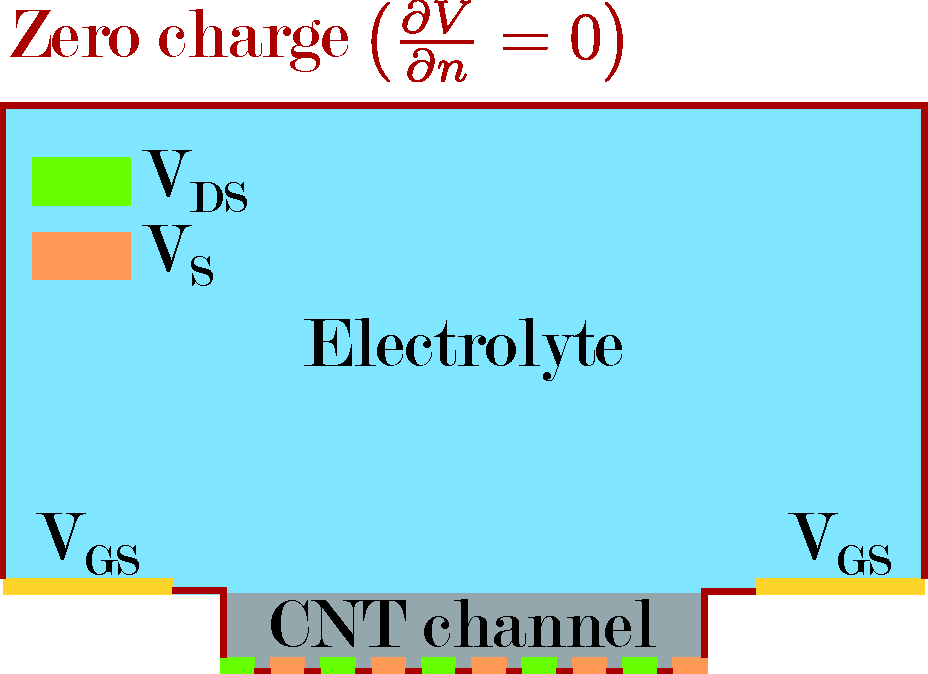
\includegraphics[width=\textwidth]{figures/chapter1/simulations/Fig7_boundaries1.pdf}
%     \end{minipage}
%     \hspace{10pt}
%     \begin{minipage}{0.3\textwidth}
%         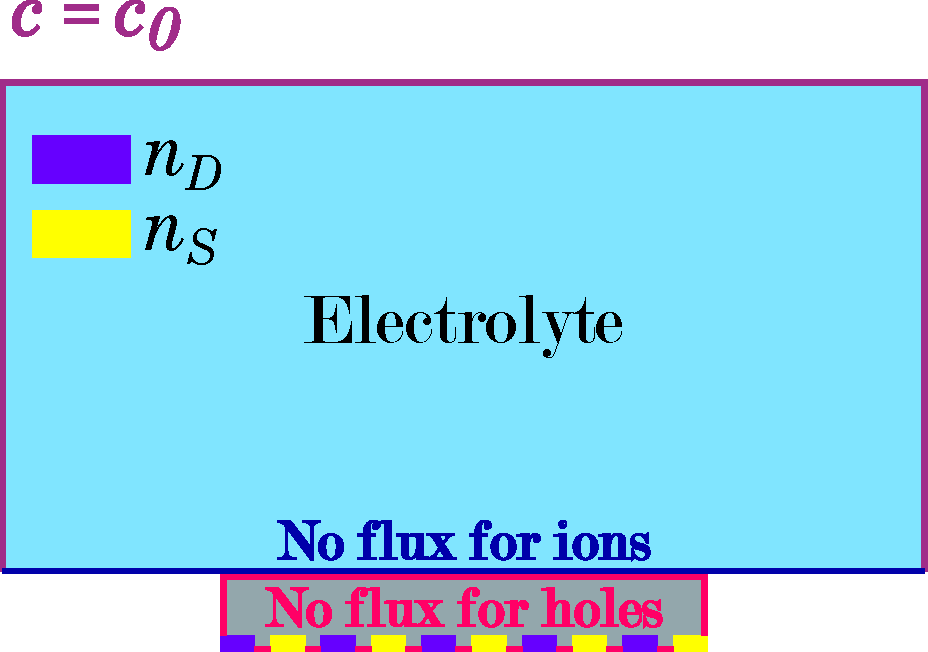
\includegraphics[width=\textwidth]{figures/chapter1/simulations/Fig7_boundaries2.pdf}
%     \end{minipage}
%     \caption{\note{Graphical representation of the boundary conditions as described in the text. The illustration highlights the constraints and parameters applied at the system's boundaries, which define the physical or mathematical behavior of the model.}}
%     \label{fig:boundaryConditions}
% \end{figure}

% In order to solve the partial differential equations above, it is necessary to establish some boundary conditions. These boundary conditions specify the constraints or values that the solution must satisfy at the boundaries of the domain under consideration. They ensure that the problem is well-posed and enable the computation of an existing and physically meaningful solution. Without these constraints, the equations cannot be solved uniquely, as multiple or infinite solutions may satisfy the governing equations.

% In the case of EG-FETs, the following boundary conditions must be established: the source is grounded, \ie{} $\mathrm{V_S} =$ \SI{0}{V}, while the gate and the drain have the voltages $\mathrm{V_G}$ and $\mathrm{V_D}$, respectively, whose values are assigned on the basis of the experiments carried out and which vary according to the type of simulation conducted. Outside the electrodes, the electric potential is zero:
% %
% \begin{displaymath}
%     \dfrac{\partial V}{\partial N} = 0.
% \end{displaymath}

% Since there is no penetration of charges from the electrolyte to the semiconductor and vice versa, it is necessary to indicate the absence of hole and ion flux at the interface between the two materials. The concentration of holes at the source and drain must also be included among the boundary conditions as follows:
% %
% \begin{equation}
%     n_S = n_0; n_D = n_S \exp\left(-\dfrac{eV_{DS}}{k_BT}\right),
% \end{equation}

% where $n_0$ is a constant indicating the initial concentration of holes at the source, $V_{DS}$ is the drain voltage, $e$ is the elementary charge, $k_B$ is the Boltzmann constant, and $T$ is the temperature; this condition thus takes into account the voltage that is applied between source and drain and updates the concentration of holes on the electrodes accordingly. For more clarity, please refer to Figure \ref{fig:boundaryConditions}

% For EG-FETs, it is important to consider that during operation (and consequently during simulations), charges move and generate two EDLs at the interface between the semiconductor and the electrolyte, and between the gate and the electrolyte. In Section~\ref{sec:EGFET}, it was described that the EDLs work as two parallel plates of a capacitor, whose specific capacitance is described by the Helmholtz equation \citep{kimElectrolyteGated2013}:
% %
% \begin{equation}
%     c = \dfrac{k\varepsilon_0}{\lambda_D},
% \end{equation}

% where $k$ is the relative permittivity of the electrolyte, $\varepsilon_0$ is the vacuum permittivity, and $\lambda_D$ is the Debye length. The latter is the quantity that describes the distance within an electrolyte over which the electric field generated by charges is screened by opposite charges present in the medium. In practical terms, it is the distance between the interface (both electrolyte-gate and electrolyte-semiconductor channel) and the outermost layer of ions, beyond which the surface charge has no effect \citep{nakatsukaAptamer2018}. The Debye length depends on various factors, such as temperature, ion density, and ionic strength (\ie{}, the salt concentration in the solution), and is defined as follows \citep{shkodraElectrolytegated2021}:
% \begin{equation}
%     \lambda_D = \sqrt{\dfrac{\varepsilon_r \varepsilon_0 k_B T}{2N_Aq^2I}},
% \end{equation}

% where $\varepsilon_0$ is the permittivity of free space, $\varepsilon_r$ is the relative permittivity of the medium, $k_B$ is the Boltzmann constant, $T$ is the temperature, $N_A$ is Avogadro's number, $q$ is the elementary charge, and $I$ is the ionic strength of the electrolyte.

% Depending on the electrolyte used, the diffusion coefficient $D_p$ and the mobility of the charges $\mu_p$ may also vary, influencing how the charges move within the medium. These two quantities are related to each other by the Nernst-Einstein relation, formulated as follows \citep{delavariNernst2021}:
% %
% \begin{equation}
%     \mu_p = \dfrac{D_p}{RT}.
% \end{equation}
% %
% Once the movement of the charges within the electrolyte is understood, it is also necessary to account for the electric field applied to the field-effect transistor, which also influences the movement of the charges. To describe these movements, the Poole-Frenkel model is used \citep{gillDrift1972,delavariNernst2021}:
% %
% \begin{equation}
%     \mu = \mu_p\exp\left(\dfrac{\gamma \sqrt{E}}{k_BT}\right),
% \end{equation}
% %
% where $\gamma$ is the Poole-Frenkel constant, and $E$ is the electric field, given by $E = \frac{V_{DS}}{d_{SD}}$. This shows how the mobility $\mu$ depends on the applied $V_{DS}$ and the distance between the source and drain.

% Having defined the operating mechanism of field-effect transistors, the next step is to evaluate their performance, that is, to calculate the output current. To this end, it is important to remember that there are two operating modes that depend on the applied voltages \citep{shkodraElectrolytegated2021}:

% \begin{itemize}
%     \item When $\lvert V_{DS} \rvert < \lvert V_{GS} \rvert - V_{th}$, the EG-FET operates in the linear regime. In this case, the current is calculated as in Equation \eqref{eq:ids_lin}:
%     \begin{equation}
%         \label{eq:ids_lin}
%         I_{DS,lin} = \mu C_{EDL}\,\frac{W}{L}\left(V_{GS}-V_{th}\right)V_{DS}
%     \end{equation}
%     \item When $\lvert V_{DS} \rvert > \lvert V_{GS} \rvert - V_{th}$, the EG-FET is said to operate in the saturation regime. In this case, the current is calculated differently, as indicated in Equation \eqref{eq:ids_sat}:
%     \begin{equation}
%         \label{eq:ids_sat}
%         I_{DS,sat} = \mu C_{EDL}\,\frac{W}{2L}\left(V_{GS}-V_{th}\right)^2
%     \end{equation}
% \end{itemize}
% %
% In the case of modeling EG-FETs and in the simulations performed, the calculation of \ids{} for the evaluation of the device performance was carried out differently; in fact, the current can be calculated by integrating the hole flux $J_p$ along the length of the channel, as shown in equation \eqref{eq:ids_int} \citep{newmanElectrochemical2021, chennitInkjetPrinted2023}:
% %
% \begin{equation}
%     \label{eq:ids_int}
%     I_{DS} = W \int_{0}^{l}J_p dl
%  \end{equation}
% %
% In addition to the drain current equations, an important parameter to evaluate the performance of EG-FETs is the transconductance ($g_m$), which quantifies the amount of current in output relative to changes in the input voltage $\left(\frac{I_{out}}{V_{in}} \right)$. For EG-FETs, it is defined as:
% %
% \begin{equation}
%     \label{eq:transconductance}
%     g_m = \mu C_{\text{ox}} \frac{W}{L} (V_{GS} - V_{th}),
% \end{equation}
% %
% where $C_{\text{ox}}$ is the oxide capacitance per unit gate area, $W$ is the channel width, and $L$ is the channel length. This equation indicates well how the transconductance depends on both material properties and device geometry, thus influencing the sensitivity and signal amplification in sensing applications.

% \subsection{Finite Element Method}
% \label{sec:FEM}
% The Finite Element Method (FEM) is a computational technique used to aaproximate the solution of nonlinear problems, especially in the fields of mechanical and electronic engineering, fluid dynamics, and related fields \citep{zienkiewiczFinite2013}. The underlying principle is to discretize the domain of partial differential equations (PDEs) into smaller elements, enabling analysis of structures, fields, and electromagnetic problems \citep{loggAutomating2007}. This discretization occurs by dividing each domain of the object under investigation into many, yet finite, smaller elements (hence the name Finite Element Method), typically segments, or triangles and squares, or tetrahedrons and cubes, depending on the shape and dimensionality of the model \citep{comsolCOMSOL_manual}. It is important to note that the elements are interconnected by nodal points, boundary lines, or surfaces, depending on the dimensionality of the problem, at which points equations governing their interactions are solved. This discretization process is commonly referred to as meshing. Once the mesh is created, each element is assigned a set of properties that depend on the type of problem being solved, including material type, electrical conductivity, charge mobility, salt concentration, and more. With these operations, a linear system of equations is generated, and boundary conditions are set to solve them. At this point, the system is solved using numerical methods for each of the previously generated elements. The elemental solutions are finally combined to provide the global solution of the system \citep{zienkiewiczFinite2013}.

% \subsubsection{COMSOL: A tool for finite element modeling and solving}
% The FEM explained in Section \ref{sec:FEM} is useful for solving complex problems, with PDEs that need to be applied to thousands, possibly millions, of elements. To address this issue and facilitate the setup, several modeling and simulation software tools have been developed, one of the most widely used being COMSOL Multiphysics \citep{comsolCOMSOL_manual}.

% \paragraph{Multiphysics}
% COMSOL offers a multiphysics platform that allows users to simulate a wide range of physical phenomena by combining different physical models, including, but not limited to, electrochemistry, charge transport, heat transfer, fluid dynamics and many more \citep{comsolCOMSOL_manual}. Other than the physics modules, the COMSOL model builder allows to choose the most appropriate space dimension for the simulations, offering one-dimensional (1D), two-dimensional (2D), and three-dimensional (3D) models \citep{comsolCOMSOL_manual}. These features make it ideal to model EG-FET devices, as they allow the coupling of the electrical and chemical processes that govern their operation through the pre-installed modules that already contain the needed system of equations, namely the \emph{Electrostatics} and the \emph{Transport of Diluted Species} modules \citep{delavariNernst2021}; moreover, they allow to simplify the problem by reducing the dimensionality to 1D of the model and build up again its complexity, as more and more knowledge is gained along the way. The power of COMSOL also lies in the fact that it is possible to simulate biological processes around the biorecognition elements (i.e., the interaction between these and the transducer, as well as the interaction between these and the analyte of interest), coupling them with the physics of the transducer, thus enabling the simulation of the operating mechanisms of a biosensor.

% \subparagraph{Electrostatics module}
% The \emph{Electrostatics} module allows the study of the electrical phenomena that govern the operation of a system. In particular, it enables the calculation of the electric field, the electric displacement field, and potential distributions in dielectric materials, within which the distribution of electric charges is known \citep{comsolCOMSOL_manual}. More specifically, the module aims to calculate the electric potential $V [V]$ as dependent variable, by solving Gauss's law for electricity \citep{grantElectromagnetism2008}:
% %
% \begin{equation}
%     \Phi_E = \dfrac{Q}{\varepsilon_0}
% \end{equation}
% %
% where $\Phi_E$ is the electric flux, which represents the amount of electric field passing through a closed surface $S$ that surrounds a volume. The total charge $Q$ contained within this volume and the electric constant $\varepsilon_0$ are also factors in this relationship. The electric flux $\Phi_E$ can also be expressed as the surface integral of the electric field over $S$ \citep{purcellElectricity2013}: %https://archive.org/details/ElectricityAndMagnetismPurcell3rdEdition/page/n101/mode/2up pag.78
% %
% \begin{equation}
%     \Phi _{E}= \oiint_S \mathbf {E} \cdot \mathrm {d} \mathbf {A}.
% \end{equation}
% %
% By the divergence theorem, Gauss's law can alternatively be written in the differential form \citep{purcellElectricity2013}: %https://archive.org/details/ElectricityAndMagnetismPurcell3rdEdition/page/n101/mode/2up pag. 80
% %
% \begin{equation}
%     \label{eq:diff_equival}
%      \nabla \mathbf{E} = \dfrac{\rho}{\varepsilon_0},
% \end{equation}
% %
% where $\nabla \mathbf{E}$ is the divergence of the electric field, $\varepsilon_0$ is the vacuum permittivity and $\rho$ is the total volume charge density (charge per unit volume).
% Equation \eqref{eq:diff_equival} is equivalent to \eqref{eq:gauss_free}, when Gauss's law is formulated in terms of free charge, rather than total charge, that is considering the charge carriers in the dielectric only \citep{griffithsIntroduction2023}:
% %
% \begin{equation}
%     \label{eq:gauss_free}
%     \nabla \mathbf{D} = \rho_f ,
% \end{equation}
% %
% where $\mathbf{D}$ is the electric displacement and $\rho_f$ is the free charge density. In isotropic medium, where the properties are the same in all directions, the displacement field $\mathbf{D}$ and the electric field $\mathbf{E}$ are related by equation \eqref{eq:displ} \citep{griffithsIntroduction2023}: % pag. 181-182-187
% \begin{equation}
%     \label{eq:displ}
%     \mathbf{D} = \varepsilon \mathbf{E} ,
% \end{equation}
% where $\varepsilon = \varepsilon_0 \varepsilon_r$.
% Finally, Gauss’s law defines how the electric field is related to charge distribution, but it doesn't specify how $\mathbf{E}$ is spatially distributed. For that, $\mathbf{E}$ needs to be connected to the electric potential $V$. Since the electric field $\mathbf{E}$ is a vector whose curl is $\mathbf{0}$, it can be equated to the gradient of a scalar, making it easier to work with. Indeed, $\mathbf{E}$ can be derived as the gradient of the electric potential \citep{griffithsIntroduction2023}: % pag. 76
% \begin{equation}
%     \label{eq:pot}
%     \mathbf{E} = -\nabla V.
% \end{equation}

% In practice, the above formulation of the problem allows to calculate the potential $V$ using boundary conditions and charge distribution. Then, \eqref{eq:pot} allows to determine field lines (or field distribution) and intensities once the charge distributions and material responses are established. Thus, this formulation allows the first part of the problem to be solved.

% \begin{remark}
% From Gauss’s law in differential form, the local charge density $\rho$ can be extrapolated and expressed as \citep{griffithsIntroduction2023}: % pag. 81

% \begin{equation}
% \rho = \nabla (-\varepsilon_0\varepsilon_r\nabla V).
% \end{equation}

% From Faraday's laws it is possible to correlate the charge density $\rho$ to the charge carrier concentration \citep{bardElectrochemical2022}. From the first law: % pag. 7

% \begin{equation}
% m = \dfrac{Q}{zF}.
% \end{equation}

% From the second law, it follows that:

% \begin{equation}
% Q = n\cdot F.
% \end{equation}

% Dividing both sides by the volume unit, it results that charge density is directly proportional to charge carrier concentration $c$:

% \begin{equation}
% \rho = c\cdot F,
% \end{equation}

% where $F$ is the Faraday constant. By assigning the charge carrier concentration $c$, it becomes possible to solve for both the electric field and the potential, completing the analysis.
% \end{remark}

% \subparagraph{Transport of Diluted Species module}
% The \emph{Transport of Diluted Species} module is dedicated to mass transfer studies, in particular to the investigation of the physical processes that regulate the transport of chemical species, them being electrons, holes, or ions, through phenomena like diffusion, convection or migration due to an electric field. In order to do so, this module calculates the concentration of species $c \left[mol/m^3\right]$ across the area or volume of the system by solving the Nernst-Planck equations presented in Section \ref{sec:simulations}. In Equation \eqref{eq:drift_el} and \eqref{eq:drift_ion}, the first term $-D_i \nabla c_i$ regulates transport by diffusion, according to Fick's law, that is driven by concentration gradients; the second term $-D_ifc_{\pm}\nabla V$ describes the drift contribution, that is, how the electric field influences charge migration and convection, which occurs when the species are carried by a flow field.

% \paragraph{Mesh}
% As explained in Section \ref{sec:FEM}, a characteristic of the finite element method is the meshing, that is the discretization of the domain of a system into smaller, finite elements. For each of these elements, a system of equations previously defined in the model will be solved. The mesh is a crucial part of the problem and great care should be used when creating one; it is indeed necessary to remember that the finer a mesh is, the more accurate the results will be, with the disadvantage of the operation being more computationally demanding, thus creating strain on the computer and requiring long solution times. The strategy that is commonly adopted is to set a very fine mesh along the boundaries, where high accuracy is required, whereas a coarser mesh is sufficient in the bulk of the domains; this evenly balances out the computational time required, without sacrificing accuracy at the boundaries. To reach the best combination of elements, the meshing process can be carried out both in a physics-controlled way, where the appropriate shape and size is automatically chosen by the sofware, or in an user-controlled way, where it can be manually set-up \citep{comsolCOMSOL_manual}.

% \paragraph{Study}
% Once the model and mesh are ready, the simulation can be launched (\emph{Study}), from which the results will be obtained. In this step, it is important to pay close attention to the settings, as they allow the choice type of study to carry out. The first key decision is whether to select a \emph{stationary} or \emph{time-dependent} study. In the first case, the simulation assumes that all conditions, such as temperature and concentration, remain constant, meaning the system is in a steady state. Mathematically, the stationary study solves equations under the assumption of time-invariance. In the second case, it is assumed that the variables change over time. These studies solve equations that include time derivatives, making them ideal for transient problems such as chemical reactions \citep{comsolCOMSOL_manual}. By setting initial conditions and observing how the system evolves over a defined time range, these studies are used to analyze processes that do not reach equilibrium instantly or exhibit time-dependent behaviour like diffusion.\\
% %
% Within this interface, it is also possible to set up parametric sweeps, such as those for electronics studies, simulating transfer and output characteristics. \\
% %
% Depending on the type of study, the most appropriate solver must be selected. Typically, COMSOL automatically selects a solver based on the aforementioned settings, yet keeping the possibility to change it manually. The options include the \emph{Automatic} solver, which detects whether a linear solver can be used, requiring no additional settings, the \emph{Linear} solver, keeps fixed Jacobians unless damping or iterations are specified, the \emph{Linear Perturbation} solver, which includes only specific weak contributions and ideal for small-signal analysis, and the \emph{Nonlinear} solver, which is designed specifically for nonlinear problems, automatically selecting suitable techniques \citep{comsolCOMSOL_manual}.
% %
% In addition to these settings, it is possible to select wheter to solve a problem with the \emph{fully coupled approach} or the \emph{segregated approach}. The former solves the entire system of equations simultaneously, accounting for all couplings in a single iteration. It requires more memory and computational power but it is often used for simpler 2D models. The latter approach breaks the problem into smaller steps, solving each step sequentially. This method reduces memory demands and is typically used for larger, more complex models like 3D simulations \citep{comsolCOMSOL_manual}.

% \paragraph{Results}
% The \emph{Results} branch in COMSOL Multiphysics provides tools to analyze and present simulation outcomes. It allows to create 1D, 2D and 3D plots and animations, conduct data analysis, and generate reports, offering a comprehensive way to interpret and share the simulation findings \citep{comsolCOMSOL_manual}.


% \note{%Mathematical modeling plays a crucial role in understanding and optimizing the behavior of electrolyte-gated field-effect transistors (EG-FETs). These devices operate through the interaction of electronic and ionic charge transport, making their analysis more complex than that of conventional field-effect transistors (FETs). The presence of an electrolyte introduces additional physical phenomena, such as electric double-layer (EDL) formation, ionic diffusion, and electrostatic screening, all of which significantly impact the device's electrical characteristics.
% Mathematical modeling plays a crucial role in understanding and optimizing the behavior of electrolyte-gated field-effect transistors (EG-FETs). These devices operate through the interaction of electronic and ionic charge transport, making their analysis more complex than that of conventional field-effect transistors (FETs). Unlike traditional FETs where the gate voltage directly modulates the channel conductivity, EG-FETs utilize an electrolyte solution to mediate the gate's influence. The presence of an electrolyte introduces additional physical phenomena, such as electric double-layer (EDL) formation, ionic diffusion, and electrostatic screening, all of which significantly impact the device's electrical characteristics. For example, the EDL, formed at the interface between the electrolyte and the gate electrode and the electrolyte and the semiconductor channel, acts as a nanoscale capacitor, influencing the gate capacitance and thus the transistor's transconductance. Ionic diffusion, governed by Fick's laws, describes the movement of ions within the electrolyte in response to concentration gradients or electric fields, affecting the EDL formation dynamics and the overall device response time. Electrostatic screening, characterized by the Debye length, describes the distance over which the electric field penetrates into the electrolyte; a shorter Debye length implies more effective screening and a stronger gate control. These phenomena are often modeled using Poisson-Nernst-Planck (PNP) equations, which couple Poisson's equation for electrostatics with the Nernst-Planck equation for ion transport. Furthermore, the semiconductor channel behavior can be modeled using drift-diffusion equations, similar to those used for conventional FETs, but with boundary conditions that account for the EDL formation and the electrochemical reactions at the semiconductor-electrolyte interface. All the equations will be provided in chapter \ref{cap:chapter5} Accurately capturing these effects in mathematical models is essential for predicting device performance, optimizing device design, and interpreting experimental results, ultimately leading to improved EG-FETs for applications in biosensing, chemical sensing, and neuromorphic computing. For instance, a well-calibrated model can predict the sensitivity of an EG-FET biosensor to a specific target molecule by simulating the change in channel current upon binding of the molecule to a receptor on the gate surface.
% %
% To accurately capture these effects, mathematical models rely on fundamental principles of electrostatics and ionic transport. Electrostatic models describe how the gate voltage modulates the charge distribution within the electrolyte and the semiconductor, often incorporating the concept of the EDL at the electrolyte/solid interface. Meanwhile, ionic transport models account for the movement of charged species within the electrolyte, influenced by diffusion, migration under an electric field, and interactions with the surrounding environment. These models provide insight into key device parameters such as threshold voltage shifts, capacitance behavior, and response times.
% \AT{Mathematical modeling plays a crucial role in understanding and optimizing the behavior of electrolyte-gated field-effect transistors (EG-FETs). These devices operate through the interaction of electronic and ionic charge transport, making their analysis more complex than that of conventional field-effect transistors (FETs). Unlike traditional FETs where the gate voltage directly modulates the channel conductivity, EG-FETs utilize an electrolyte solution to mediate the gate's influence. The presence of an electrolyte introduces additional physical phenomena, such as electric double-layer (EDL) formation, ionic diffusion, and electrostatic screening, all of which significantly impact the device's electrical characteristics. For example, the EDL, formed at the interface between the electrolyte and the gate electrode and the electrolyte and the semiconductor channel, acts as a nanoscale capacitor, influencing the gate capacitance and thus the transistor's transconductance. Ionic diffusion, governed by Fick's laws, describes the movement of ions within the electrolyte in response to concentration gradients or electric fields, affecting the EDL formation dynamics and the overall device response time. Electrostatic screening, characterized by the Debye length, describes the distance over which the electric field penetrates into the electrolyte; a shorter Debye length implies more effective screening and a stronger gate control. These phenomena are often modeled using Poisson-Nernst-Planck (PNP) equations, which couple Poisson's equation for electrostatics with the Nernst-Planck equation for ion transport. Furthermore, the semiconductor channel behavior can be modeled using drift-diffusion equations, similar to those used for conventional FETs, but with boundary conditions that account for the EDL formation and the electrochemical reactions at the semiconductor-electrolyte interface. Accurately capturing these effects in mathematical models is essential for predicting device performance, optimizing device design, and interpreting experimental results, ultimately leading to improved EG-FETs for applications in biosensing, chemical sensing, and neuromorphic computing. For instance, a well-calibrated model can predict the sensitivity of an EG-FET biosensor to a specific target molecule by simulating the change in channel current upon binding of the molecule to a receptor on the gate surface. To accurately capture these effects, mathematical models rely on fundamental principles of electrostatics and ionic transport, describing how the gate voltage modulates the charge distribution within the electrolyte and the semiconductor, often incorporating the concept of the EDL at the electrolyte/solid interface. Meanwhile, ionic transport models account for the movement of charged species within the electrolyte, influenced by diffusion, migration under an electric field, and interactions with the surrounding environment, providing insight into key device parameters such as threshold voltage shifts, capacitance behavior, and response times.}
% %
% %Given the complexity of coupled electronic and ionic interactions, numerical simulations are essential for solving the governing equations governing EGFET operation. Finite element methods (FEM) are widely used to simulate electrostatic potential distributions and charge transport, while drift-diffusion models provide a framework for analyzing carrier dynamics in the transistor channel. Additionally, molecular dynamics (MD) simulations offer insights into ion behavior at the atomic level, particularly in systems where nanoscale effects become significant. By integrating these approaches, multiscale modeling techniques aim to bridge the gap between microscopic ion transport and macroscopic electrical response.
% %
% %Simulations based on these models serve as powerful tools for optimizing EGFET performance. They enable the prediction of device behavior under different electrolyte conditions, aid in material selection, and provide guidance for experimental design. However, challenges remain in achieving a balance between computational efficiency and model accuracy, particularly when accounting for complex electrochemical interactions. Emerging techniques, such as machine learning-assisted modeling, offer promising directions for improving predictive capabilities while reducing computational costs.
% %
% %In the following sections, we present a detailed discussion of the mathematical framework governing EGFET operation, including electrostatic modeling, ionic transport equations, and numerical solution strategies.
% }

% \note{The modeling and simulation of electronic devices span a broad spectrum of techniques, each tailored to capture specific physical effects and operating scales. For devices such as electrolyte-gated field-effect transistors (EGFETs), where electrostatics, ionic transport, and semiconductor physics are tightly coupled, a variety of computational strategies are employed to understand and predict device behavior. These methods range from continuum-level numerical solvers to atomistic and data-driven approaches, depending on the complexity of the system under investigation.
% %
% One of the most commonly used techniques is the finite element method (FEM), which is particularly effective in solving partial differential equations arising from electrostatic, ionic, and carrier transport phenomena in complex geometries. Software platforms such as COMSOL Multiphysics leverage FEM to solve coupled physics problems, making it suitable for simulating the interplay between ionic motion in the electrolyte and charge modulation in the semiconductor channel. Similar to FEM, the finite difference method (FDM) offers an alternative grid-based approach for solving transport equations, often used in simpler or more structured simulation domains due to its ease of implementation.
% %
% In addition to FEM and FDM, the finite volume method (FVM) is also utilized, especially in scenarios requiring strict conservation of fluxes, such as in electrochemical systems. At the circuit level, SPICE-based simulations provide a more abstracted modeling framework, representing EGFETs as lumped components within electronic circuits. While SPICE lacks spatial resolution and cannot model ionic transport explicitly, it remains useful for system-level validation and integration studies.
% %
% For a more comprehensive representation of carrier dynamics within semiconductors, TCAD tools (Technology Computer-Aided Design), such as Synopsys Sentaurus or Silvaco Atlas, offer built-in physical models for drift-diffusion, recombination, and quantum effects. These are widely used in the semiconductor industry and research to simulate conventional FET behavior, and they can be extended or coupled with electrolyte models to capture EGFET characteristics.
% %
% At the atomistic scale, molecular dynamics (MD) simulations are employed to investigate ion behavior and solvent interactions within the electrolyte, especially at interfaces where continuum models may break down. Monte Carlo methods provide a stochastic alternative for modeling carrier transport or tunneling effects in semiconductors. More recently, machine learning and data-driven models have emerged as powerful tools for predicting device behavior from simulation or experimental datasets, offering significant computational speed-ups once trained, and enabling rapid design space exploration.
% %
% By leveraging these diverse modeling approaches—often in combination through multiscale or multiphysics frameworks—researchers can capture the full range of physical interactions governing EGFET performance. The selection of a particular simulation method is typically guided by the target application, desired level of accuracy, and available computational resources.}

% \AT{Mathematical modeling and simulation form the foundation of modern electronic device analysis and design. With the increasing complexity of electronic systems and the miniaturization of device architectures, it has become essential to employ computational approaches that can predict physical behavior, optimize performance, and reduce reliance on costly experimental iterations. These models are based on physical laws governing charge transport, electrostatics, thermodynamics, and quantum phenomena, which are translated into mathematical formulations solvable through various numerical techniques.
% %
% A range of modeling techniques is available depending on the desired level of abstraction and the physical scales involved. At the device level, continuum-based models, such as those used in Technology Computer-Aided Design (TCAD), solve systems of coupled partial differential equations—typically including Poisson’s equation and carrier transport equations like the drift-diffusion model. For systems where spatial detail and physical accuracy are critical, numerical methods such as the finite element method (FEM), finite difference method (FDM), and finite volume method (FVM) are employed. These methods are capable of handling complex geometries and coupled multiphysics scenarios, such as electro-thermal or electrochemical interactions. At finer scales, atomistic simulations like molecular dynamics (MD) or quantum mechanical models are used to capture nanoscale effects and material properties. More recently, machine learning and data-driven approaches have been introduced to complement physical models, enabling rapid approximation of device behavior and real-time optimization based on large datasets.
% %
% In this broader context, mathematical modeling plays a crucial role in understanding and optimizing the behavior of electrolyte-gated field-effect transistors (EG-FETs). These devices operate through the interaction of electronic and ionic charge transport, making their analysis more complex than that of conventional field-effect transistors. Unlike traditional FETs, where the gate voltage directly modulates the channel conductivity, EG-FETs utilize an electrolyte to mediate the gate’s influence. This introduces additional physical mechanisms—such as electric double-layer (EDL) formation, ionic diffusion, and electrostatic screening—that must be considered in the modeling framework. For instance, the EDL, formed at the interface between the electrolyte and both the gate electrode and the semiconductor channel, acts as a nanoscale capacitor, strongly influencing the gate capacitance and transconductance. Ionic diffusion, governed by concentration gradients and electric fields, affects the dynamics of EDL formation and the device’s transient response. Electrostatic screening, typically characterized by the Debye length, dictates the extent to which the electric field penetrates the electrolyte and influences the semiconductor channel.
% %
% To accurately capture these effects, mathematical models rely on fundamental principles of electrostatics and ionic transport. These models often incorporate concepts such as the Poisson–Nernst–Planck framework to describe the coupling between ion transport and electrostatic potential in the electrolyte, and drift-diffusion models to represent carrier dynamics in the semiconductor channel. Boundary conditions at the electrolyte/semiconductor interface must account for EDL formation and possible electrochemical reactions. Together, these models enable the prediction of key device parameters—such as threshold voltage shifts, gate capacitance variations, and transient current responses—and support the development of EG-FETs for a wide range of applications, including biosensing, chemical detection, and neuromorphic computing.
% %
% All governing equations and numerical formulations used in this study are presented in detail in Chapter \ref{cap:chapter5}.}

Mathematical modeling and simulation are fundamental complementary activities in modern electronics, especially useful for device analysis and design. With the increasing complexity of electronic systems and the miniaturization of device architectures, the computational approaches can help to predict physical behavior, optimize performance, and reduce the number of experiments needed \citep{markowichDrift1990}. For example, simulating a complex integrated circuit with billions of transistors allows engineers to identify potential bottlenecks and optimize power consumption before fabrication, saving significant time and resources \citep{zandShortChannel2020}. Consider the design of a high-performance microprocessor; without simulation, optimizing the placement of billions of transistors to minimize signal delay and power dissipation would be virtually impossible. In the semiconductor industry, numerical simulation aims to replace as much laboratory testing as possible to minimize costs. Physically detailed simulations are crucial for addressing challenges in nanoscale devices, capturing off-equilibrium transport and quantum mechanical effects \citep{hayatiCNTMOSFET2010}. Moreover, with the increased miniaturization of semiconductor devices, simulation becomes even more important as physical limits are approached and quantum mechanical effects play a larger role \citep{zandShortChannel2020}. 
These models are based on physical laws governing charge transport, electrostatics, thermodynamics, and quantum phenomena, which are translated into mathematical formulations solvable through various numerical techniques \citep{delavariNernst2021,hassaniniaSimulation2008,moghadamDesign2013}. A range of modeling techniques is available depending on the desired level of abstraction and the physical scales involved. 

At the device level, continuum-based models, such as those used in Technology Computer-Aided Design (TCAD), solve systems of coupled partial differential equations, typically including Poisson's equation and carrier transport equations like the drift-diffusion model \citep{markowichDrift1990}. Poisson's equation describes the electrostatic potential distribution based on charge density \citep{delavariNernst2021}, while the drift-diffusion model describes the movement of charge carriers (electrons and holes) under the influence of electric fields and concentration gradients \citep{markowichDrift1990}. TCAD tools like Synopsys Sentaurus and Silvaco Atlas are widely used in the semiconductor industry to simulate transistor behavior and optimize device fabrication processes \citep{tungaPhysicsBased2023}. For instance, TCAD simulations can be used to optimize the doping profiles in a MOSFET to achieve desired threshold voltage and on-current characteristics.  In the context of Carbon Nanotube Field-Effect Transistors (CNTFETs), the self-consistent solution of the Poisson and Schrödinger equations using the Non-Equilibrium Green's Function (NEGF) formalism is a common approach, demonstrating the application of these fundamental equations at the nanoscale \citep{hassaniniaSimulation2008,zandShortChannel2020}. 

For systems where spatial detail and physical accuracy are critical, numerical methods such as the finite element method (FEM) and finite difference method (FDM) are employed \citep{jagotaFinite2013,moghadamDesign2013}. These methods are capable of handling complex geometries and coupled multiphysics scenarios, such as electro-thermal or electrochemical interactions \citep{jagotaFinite2013,drummondLoworder2015}. For instance, FEM can be used to simulate heat transfer, which is crucial for understanding the temperature distribution within a device where electrical power dissipation generates heat and the thermal conductivity of the materials influences heat flow \citep{jagotaFinite2013}. This type of analysis is essential for preventing thermal runaway and ensuring reliable operation. The finite difference method (FDM) is also used for numerical solutions in device modeling, such as discretizing the Poisson equation to determine the electrostatic potential and in simulating electrochemical devices like supercapacitors \citep{moghadamDesign2013,drummondLoworder2015}. 

At finer scales, atomistic simulations like molecular dynamics (MD) or quantum mechanical models are used to understans nanoscale effects and material properties \citep{hayatiCNTMOSFET2010}. MD simulations, using software like LAMMPS or GROMACS, can predict the behavior of atoms in a transistor channel, revealing insights into electron mobility and scattering mechanisms. For example, MD simulations can be used to study the impact of surface roughness on electron transport in nanoscale transistors \citep{zhaoUnderstanding2018}.

Density Functional Theory (DFT) is a common quantum mechanical method used to calculate the electronic structure of materials and predict their properties. DFT calculations can be used to determine the band structure of a semiconductor material or to predict the binding energy of molecules on a surface \citep{xiaoAccurate2011}. More recently, machine learning and data-driven approaches have been introduced to complement physical models, enabling rapid approximation of device behavior and real-time optimization based on large datasets. For example, \citet{hayatiCNTMOSFET2010} explored an artificial neural network approach for the modeling and simulation of carbon nanotube metal oxide-semiconductor field-effect transistors (CNT MOSFETs).  In this work, a numerical model of the current-voltage characteristics, derived from 2-D numerical Non-Equilibrium Green's Function (NEGF) simulation, was used to generate the required database for optimizing the proposed ANN model. The NEGF formalism itself involves the self-consistent solution of the Poisson and Schrödinger equations and is a sound approach for simulating non-equilibrium nanoscale systems like CNTFETs. The aim of using ANNs is to develop fast methods that can be implemented in SPICE-type circuit simulators, where high computational speed is necessary due to the complexity and time-consuming nature of full numerical analyses using methods like NEGF. Therefore, neural networks can be trained on data obtained from such numerical simulations to quickly predict device performance under different operating conditions, potentially accelerating the design process by allowing for rapid exploration of device parameters.

In this broader context, mathematical modeling plays a crucial role in understanding and optimizing the behavior of EG-FETs. These devices operate through the interaction of electronic and ionic charge transport, making their analysis more complex than that of conventional field-effect transistors. Unlike traditional FETs, where the gate voltage directly modulates the channel conductivity, EG-FETs utilize an electrolyte to mediate the influence of the gate \citep{delavariNernst2021,chennitInkjetPrinted2023}. This introduces additional physical mechanisms—such as electric double-layer (EDL) formation, ionic diffusion, and electrostatic screening—that must be considered in the modeling framework \citep{delavariNernst2021,chennitInkjetPrinted2023}. For instance, the EDL, formed at the interface between the electrolyte and both the gate electrode and the semiconductor channel, acts as a nanoscale capacitor, strongly influencing the gate capacitance and transconductance \citep{masseyModeling2021}. The overall capacitive coupling between the gate electrode and the organic semiconductor in EG-FETs can be described as a series of capacitors associated with the gate/electrolyte and electrolyte/semiconductor interfaces. Moreover, unlike traditional MOSFETs with a solid dielectric, the capacitive coupling in EG-FETs is ensured through the electrolyte, which is characterized by mobile ionic charges and the formation of EDLs \citep{delavariNernst2021,piccaUltimately2020}. 
The capacitance of the EDL can be modeled using the Gouy-Chapman-Stern theory, which accounts for the ionic concentration profile near the interface. The Gouy-Chapman-Stern model explicitly describes two distinct regions: the inner Stern layer and the outer diffuse layer, combining aspects of the earlier Helmholtz and Gouy-Chapman models. In the diffuse layer, the ions are mobile and their distribution is influenced by both diffusion driven by concentration gradients and electromigration driven by the electric potential gradient. The Stern layer accounts for the finite size of ions. The overall capacitance can be considered as a series combination of the Stern layer capacitance and the diffuse layer capacitance \citep{pilonRecent2015}.
Consequently, models for EG-FETs need to account for the redistribution of ions within the electrolyte upon gate polarization \citep{delavariNernst2021,pilonRecent2015}. Indeed, ionic diffusion, governed by concentration gradients and electric fields, affects the dynamics of EDL formation and the device's transient response. Furthermore, the diffusion coefficient of ions in the electrolyte is a crucial parameter that influences the speed of the device and their ability to dissociate and serve as free charge carriers. Using an electrolyte with a larger ionic conductivity and mobility, which are related to the diffusion coefficient, generally leads to faster charge-discharge rates in devices. The time-dependent properties of different electrolyte forms, including their diffusion characteristics, are important for understanding the transient behavior of electrolyte capacitors and electrolyte-gated devices \citep{masseyModeling2021}.
Additionally, electrostatic screening must be considered, as thoroughly described by \citet{delavariNernst2021}. This is typically characterized by the Debye length, and dictates the extent to which the electric field penetrates the electrolyte and influences the semiconductor channel. A shorter Debye length implies stronger screening and a more localized gate effect. Indeed, for a small gate EG-FET, stronger screening at the gate-electrolyte interface due to its smaller area leads to a negligible potential drop and electric field at the polymer/electrolyte interface, thus limiting the gate's influence on the channel. Conversely, when the electrolyte concentration is lower, the gate is poorly screened, and the transistor action is partially restored, indicating that stronger screening hinders the field effect. The Debye length is inversely proportional to the square root of the ionic concentration. This means that higher ionic concentrations lead to a smaller Debye length and stronger screening. 

These models often incorporate concepts such as the Poisson-Nernst-Planck framework to describe the coupling between ion transport and electrostatic potential in the electrolyte, and drift-diffusion models to represent carrier dynamics in the semiconductor channel. In the context of EG-FETs, models utilizing the Nernst-Planck-Poisson (NPP) equations treat both the polymer and the electrolyte regions on an equal footing, allowing for a quantitative description of their electrical characteristics \citep{delavariNernst2021,chennitInkjetPrinted2023}. These equations account for the electrostatics of the system as well as the transport of all the charged species involved. Hole transport in the organic semiconductor region can be described by a drift-diffusion equation that includes both diffusion and drift contributions, coupled with the Poisson equation which describes the electrostatic potential. Similarly, ion transport in the electrolyte is described by the Nernst-Planck equations, considering positive and negative ions as charged species, also coupled with the Poisson equation \citep{delavariNernst2021,chennitInkjetPrinted2023}.
The Poisson-Nernst-Planck equations are a set of coupled partial differential equations that describe the distribution of ions and the electric potential in an electrolyte solution. The Poisson equation relates the electric potential to the charge density through the permittivity. The charge density in the electrolyte is determined by the concentrations of positive and negative ions. In the semiconductor, it relates to the hole concentration.
The Nernst-Planck equation describes the flux of ions due to diffusion (proportional to the concentration gradient) and electromigration (driven by the electric field). With this equation it is possible to highlight the coupling between the movement of ions and the electric field within the electrolyte \citep{delavariNernst2021,chennitInkjetPrinted2023}.
Furthermore, the drift-diffusion equation used for the semiconductor region expresses the current density as a sum of drift and diffusion contributions corresponding to the migration of charge carriers in an electric field and the flux due to concentration gradient, respectively. The mobility of charge carriers in the semiconductor is often related to the diffusion coefficient by the Nernst-Einstein relation. Boundary conditions at the electrolyte/semiconductor interface must account for electric double layer (EDL) formation and possible electrochemical reactions \citep{delavariNernst2021,chennitInkjetPrinted2023}. 

Together, these models enable the prediction of key device parameters—such as threshold voltage shifts, gate capacitance variations, and transient current responses; thanks to this, they can support the development of EG-FETs for a wide range of applications, from biosensing \citep{piccaUltimately2020,chennitInkjetPrinted2023}, to neuromorphic computing \citep{masseyModeling2021}.
In biosensing, EG-FETs can detect the presence of specific biomolecules by measuring changes in the device's electrical characteristics upon binding of the target molecule to the gate surface. For example, an EG-FET can be functionalized with antibodies that specifically bind to a target analyte, and the binding event can be detected as a change in the drain current \citep{piccaUltimately2020}. In neuromorphic computing, EG-FETs can be used to mimic the behavior of biological synapses, enabling the development of energy-efficient artificial neural networks. The gradual change in conductance of an EG-FET in response to a series of voltage pulses can mimic the synaptic plasticity observed in biological neurons \citep{masseyModeling2021}.

\subsection{Finite Element Method}
\label{sec:FEM}
The Finite Element Method (FEM) is a computational technique used to aaproximate the solution of nonlinear problems, especially in the fields of mechanical and electronic engineering, fluid dynamics, and related fields \citep{zienkiewiczFinite2013}. The underlying principle is to discretize the domain of partial differential equations (PDEs) into smaller elements, enabling analysis of structures, fields, and electromagnetic problems \citep{loggAutomating2007}. This discretization occurs by dividing each domain of the object under investigation into many, yet finite, smaller elements (hence the name Finite Element Method), typically segments, or triangles and squares, or tetrahedrons and cubes, depending on the shape and dimensionality of the model \citep{comsolCOMSOL_manual}. It is important to note that the elements are interconnected by nodal points, boundary lines, or surfaces, depending on the dimensionality of the problem, at which points equations governing their interactions are solved. This discretization process is commonly referred to as meshing. Once the mesh is created, each element is assigned a set of properties that depend on the type of problem being solved, including material type, electrical conductivity, charge mobility, salt concentration, and more. With these operations, a linear system of equations is generated, and boundary conditions are set to solve them. At this point, the system is solved using numerical methods for each of the previously generated elements. The elemental solutions are finally combined to provide the global solution of the system \citep{zienkiewiczFinite2013}.

\subsubsection{COMSOL: A tool for finite element modeling and solving}
The FEM explained in Section \ref{sec:FEM} is useful for solving complex problems, with PDEs that need to be applied to thousands, possibly millions, of elements. To address this issue and facilitate the setup, several modeling and simulation software tools have been developed, one of the most widely used being COMSOL Multiphysics \citep{comsolCOMSOL_manual}.

\paragraph{Multiphysics}
COMSOL offers a multiphysics platform that allows users to simulate a wide range of physical phenomena by combining different physical models, including, but not limited to, electrochemistry, charge transport, heat transfer, fluid dynamics and many more \citep{comsolCOMSOL_manual}. Other than the physics modules, the COMSOL model builder allows to choose the most appropriate space dimension for the simulations, offering one-dimensional (1D), two-dimensional (2D), and three-dimensional (3D) models \citep{comsolCOMSOL_manual}. These features make it ideal to model EG-FET devices, as they allow the coupling of the electrical and chemical processes that govern their operation through the pre-installed modules that already contain the needed system of equations, namely the \emph{Electrostatics} and the \emph{Transport of Diluted Species} modules \citep{delavariNernst2021}; moreover, they allow to simplify the problem by reducing the dimensionality to 1D of the model and build up again its complexity, as more and more knowledge is gained along the way. The power of COMSOL also lies in the fact that it is possible to simulate biological processes around the biorecognition elements (i.e., the interaction between these and the transducer, as well as the interaction between these and the analyte of interest), coupling them with the physics of the transducer, thus enabling the simulation of the operating mechanisms of a biosensor.

\subparagraph{Electrostatics module}
The \emph{Electrostatics} module allows the study of the electrical phenomena that govern the operation of a system. In particular, it enables the calculation of the electric field, the electric displacement field, and potential distributions in dielectric materials, within which the distribution of electric charges is known \citep{comsolCOMSOL_manual}. More specifically, the module aims to calculate the electric potential $V [V]$ as dependent variable, by solving Gauss's law for electricity \citep{grantElectromagnetism2008}:
%
\begin{equation}
    \Phi_E = \dfrac{Q}{\varepsilon_0}
\end{equation}
%
where $\Phi_E$ is the electric flux, which represents the amount of electric field passing through a closed surface $S$ that surrounds a volume. The total charge $Q$ contained within this volume and the electric constant $\varepsilon_0$ are also factors in this relationship. The electric flux $\Phi_E$ can also be expressed as the surface integral of the electric field over $S$ \citep{purcellElectricity2013}: %https://archive.org/details/ElectricityAndMagnetismPurcell3rdEdition/page/n101/mode/2up pag.78
%
\begin{equation}
    \Phi _{E}= \oiint_S \mathbf {E} \cdot \mathrm {d} \mathbf {A}.
\end{equation}
%
By the divergence theorem, Gauss's law can alternatively be written in the differential form \citep{purcellElectricity2013}: %https://archive.org/details/ElectricityAndMagnetismPurcell3rdEdition/page/n101/mode/2up pag. 80
%
\begin{equation}
    \label{eq:diff_equival}
     \nabla \mathbf{E} = \dfrac{\rho}{\varepsilon_0},
\end{equation}
%
where $\nabla \mathbf{E}$ is the divergence of the electric field, $\varepsilon_0$ is the vacuum permittivity and $\rho$ is the total volume charge density (charge per unit volume).
Equation \eqref{eq:diff_equival} is equivalent to \eqref{eq:gauss_free}, when Gauss's law is formulated in terms of free charge, rather than total charge, that is considering the charge carriers in the dielectric only \citep{griffithsIntroduction2023}:
%
\begin{equation}
    \label{eq:gauss_free}
    \nabla \mathbf{D} = \rho_f ,
\end{equation}
%
where $\mathbf{D}$ is the electric displacement and $\rho_f$ is the free charge density. In isotropic medium, where the properties are the same in all directions, the displacement field $\mathbf{D}$ and the electric field $\mathbf{E}$ are related by equation \eqref{eq:displ} \citep{griffithsIntroduction2023}: % pag. 181-182-187
\begin{equation}
    \label{eq:displ}
    \mathbf{D} = \varepsilon \mathbf{E} ,
\end{equation}
where $\varepsilon = \varepsilon_0 \varepsilon_r$.
Finally, Gauss’s law defines how the electric field is related to charge distribution, but it doesn't specify how $\mathbf{E}$ is spatially distributed. For that, $\mathbf{E}$ needs to be connected to the electric potential $V$. Since the electric field $\mathbf{E}$ is a vector whose curl is $\mathbf{0}$, it can be equated to the gradient of a scalar, making it easier to work with. Indeed, $\mathbf{E}$ can be derived as the gradient of the electric potential \citep{griffithsIntroduction2023}: % pag. 76
\begin{equation}
    \label{eq:pot}
    \mathbf{E} = -\nabla V.
\end{equation}

In practice, the above formulation of the problem allows to calculate the potential $V$ using boundary conditions and charge distribution. Then, \eqref{eq:pot} allows to determine field lines (or field distribution) and intensities once the charge distributions and material responses are established. Thus, this formulation allows the first part of the problem to be solved.

\begin{remark}
From Gauss’s law in differential form, the local charge density $\rho$ can be extrapolated and expressed as \citep{griffithsIntroduction2023}: % pag. 81

\begin{equation}
\rho = \nabla (-\varepsilon_0\varepsilon_r\nabla V).
\end{equation}

From Faraday's laws it is possible to correlate the charge density $\rho$ to the charge carrier concentration \citep{bardElectrochemical2022}. From the first law: % pag. 7

\begin{equation}
m = \dfrac{Q}{zF}.
\end{equation}

From the second law, it follows that:

\begin{equation}
Q = n\cdot F.
\end{equation}

Dividing both sides by the volume unit, it results that charge density is directly proportional to charge carrier concentration $c$:

\begin{equation}
\rho = c\cdot F,
\end{equation}

where $F$ is the Faraday constant. By assigning the charge carrier concentration $c$, it becomes possible to solve for both the electric field and the potential, completing the analysis.
\end{remark}

\subparagraph{Transport of Diluted Species module}
The \emph{Transport of Diluted Species} module is dedicated to mass transfer studies, in particular to the investigation of the physical processes that regulate the transport of chemical species, them being electrons, holes, or ions, through phenomena like diffusion, convection or migration due to an electric field. In order to do so, this module calculates the concentration of species $c \left[mol/m^3\right]$ across the area or volume of the system by solving the Nernst-Planck equations presented in Section \ref{sec:simulations}. In Equation \eqref{eq:drift_el} and \eqref{eq:drift_ion}, the first term $-D_i \nabla c_i$ regulates transport by diffusion, according to Fick's law, that is driven by concentration gradients; the second term $-D_ifc_{\pm}\nabla V$ describes the drift contribution, that is, how the electric field influences charge migration and convection, which occurs when the species are carried by a flow field.

\paragraph{Mesh}
As explained in Section \ref{sec:FEM}, a characteristic of the finite element method is the meshing, that is the discretization of the domain of a system into smaller, finite elements. For each of these elements, a system of equations previously defined in the model will be solved. The mesh is a crucial part of the problem and great care should be used when creating one; it is indeed necessary to remember that the finer a mesh is, the more accurate the results will be, with the disadvantage of the operation being more computationally demanding, thus creating strain on the computer and requiring long solution times. The strategy that is commonly adopted is to set a very fine mesh along the boundaries, where high accuracy is required, whereas a coarser mesh is sufficient in the bulk of the domains; this evenly balances out the computational time required, without sacrificing accuracy at the boundaries. To reach the best combination of elements, the meshing process can be carried out both in a physics-controlled way, where the appropriate shape and size is automatically chosen by the sofware, or in an user-controlled way, where it can be manually set-up \citep{comsolCOMSOL_manual}.

\paragraph{Study}
Once the model and mesh are ready, the simulation can be launched (\emph{Study}), from which the results will be obtained. In this step, it is important to pay close attention to the settings, as they allow the choice type of study to carry out. The first key decision is whether to select a \emph{stationary} or \emph{time-dependent} study. In the first case, the simulation assumes that all conditions, such as temperature and concentration, remain constant, meaning the system is in a steady state. Mathematically, the stationary study solves equations under the assumption of time-invariance. In the second case, it is assumed that the variables change over time. These studies solve equations that include time derivatives, making them ideal for transient problems such as chemical reactions \citep{comsolCOMSOL_manual}. By setting initial conditions and observing how the system evolves over a defined time range, these studies are used to analyze processes that do not reach equilibrium instantly or exhibit time-dependent behaviour like diffusion.\\
%
Within this interface, it is also possible to set up parametric sweeps, such as those for electronics studies, simulating transfer and output characteristics. \\
%
Depending on the type of study, the most appropriate solver must be selected. Typically, COMSOL automatically selects a solver based on the aforementioned settings, yet keeping the possibility to change it manually. The options include the \emph{Automatic} solver, which detects whether a linear solver can be used, requiring no additional settings, the \emph{Linear} solver, keeps fixed Jacobians unless damping or iterations are specified, the \emph{Linear Perturbation} solver, which includes only specific weak contributions and ideal for small-signal analysis, and the \emph{Nonlinear} solver, which is designed specifically for nonlinear problems, automatically selecting suitable techniques \citep{comsolCOMSOL_manual}.
%
In addition to these settings, it is possible to select wheter to solve a problem with the \emph{fully coupled approach} or the \emph{segregated approach}. The former solves the entire system of equations simultaneously, accounting for all couplings in a single iteration. It requires more memory and computational power but it is often used for simpler 2D models. The latter approach breaks the problem into smaller steps, solving each step sequentially. This method reduces memory demands and is typically used for larger, more complex models like 3D simulations \citep{comsolCOMSOL_manual}.

\paragraph{Results}
The \emph{Results} branch in COMSOL Multiphysics provides tools to analyze and present simulation outcomes. It allows to create 1D, 2D and 3D plots and animations, conduct data analysis, and generate reports, offering a comprehensive way to interpret and share the simulation findings \citep{comsolCOMSOL_manual}.